\documentclass[10pt, letterpaper]{article}
\usepackage{listings}
\usepackage[utf8]{inputenc}
\usepackage{graphicx}
\usepackage{xcolor}
\usepackage{float}
\graphicspath{ {./images/}  }

\definecolor{codegreen}{rgb}{0,0.6,0}
\definecolor{codegray}{rgb}{0.5,0.5,0.5}
\definecolor{codepurple}{rgb}{0.58,0,0.82}
\definecolor{backcolour}{rgb}{0.93,0.95,0.92}

\lstdefinestyle{mystyle}{
    backgroundcolor=\color{backcolour},   
    commentstyle=\color{codegreen},
    keywordstyle=\color{magenta},
    numberstyle=\tiny\color{codegray},
    stringstyle=\color{codepurple},
    basicstyle=\ttfamily\footnotesize,
    breakatwhitespace=false,         
    breaklines=true,                 
    captionpos=b,                    
    keepspaces=true,                 
    numbers=left,                    
    numbersep=5pt,                  
    showspaces=false,                
    showstringspaces=false,
    showtabs=false,                  
    tabsize=2
}

\lstset{style=mystyle}

\emergencystretch 5em%
\newcommand{\code}[1]{\texttt{#1}}
\newcommand{\dline}{\par\noindent\rule{\textwidth}{0.2pt}\\}
\usepackage[margin=1in]{geometry}

\title{COMP 421 - Database Systems \\ 
\large Project 2: Database Creation}
\author{Seyed Yazdan Zinati\\seyed.zinati@mail.mcgill.ca\\ 260928077}
\date{\today}

\begin{document}
\maketitle

\section*{Relational Model}
The relational model has not been modified from Project 1 with the exception of replacing \code{date} and \code{time} columns in the \code{Note} table by \code{timestamp}.
\subsection*{Model}
\dline
\code{HealthcareInstitution(\underline{hcId}, phoneNum, name, email, address, website)}
\dline
\code{CommunityClinic(\underline{hcId})}\\
\\
\code{hcId} foreign key referencing \code{HealthcareInstitution}
\dline
\code{BirthingCenter(\underline{hcId})}\\
\\
\code{hcId} foreign key referencing \code{HealthcareInstitution}
\dline
\code{Midwife(\underline{pracId}, name, email, phoneNum, hcId)}\\
\\
\code{hcId} foreign key referencing \code{HealthcareInstitution}\\
\\
note: \code{hcId} has to be \code{NOT NULL} to enforce Midwife's participation constraint in the \code{employs} relationship set.
\dline
\code{Father(\underline{fatherId}, phoneNum, name, email, address, QChcardid, dateOfBirth, profession, bloodType)}
\dline
\code{Mother(\underline{QChcardid}, phoneNum, name, email, adddress, dateOfBirth, profession, bloodType)}
\dline
\code{Couple(\underline{coupleId}, invited, interested, selected, QChcardid, fatherId)}\\
\\
\code{QChcardid} foreign key referencing \code{Mother}\\
\code{fatherId} foreign key referencing \code{Father}\\
\\
note: \code{QChcardid} has to be \code{NOT NULL} to enforce Couple's participation constraint in the \code{constitutesF} relationship set.

\dline
\code{InformationSession(\underline{sessId}, language, date, time, pracId)}\\
\\
\code{pracId} foreign key referencing Midwife\\
\\
note: \code{pracId} has to be \code{NOT NULL} to enforce InformationSession's participation constraint in the \code{hosts} relationship set.
\dline
\code{Invitation(\underline{sessId, coupleId}, attended, registered)}\\

\noindent\code{sessId} foreign key referencing \code{Information Session}\\
\code{coupleId} foreign key referencing \code{Couple}
\dline
\code{Pregnancy(\underline{coupleId, pregNum}, estDueDate, expBirthTimeframe, lastMenstPeriod, isHomeBirth, primaryMidwife, backupMidwife)}\\
\\
\code{coupleId} foreign key referencing \code{Couple}\\
\code{primaryMidwife} foreign key referencing \code{Midwife(pracId)}\\
\code{backupMidwife} foreign key referencing \code{Midwife(pracId)}\\
\\
note: \code{coupleId} is part of the primary key and thus has to be \code{NOT NULL}.
\dline
\code{Appointment(\underline{apptId}, date, time, pregNum, coupleId, pracId)}\\
\\
\code{(pregNum, coupleId)} foreign key referencing \code{Pregnancy}\\
\code{pracId} foreign key referencing \code{Midwife}\\
\\
note: \code{pregNum} and \code{coupleId} has to be \code{NOT NULL} to enforce Appointment's participation constraint in the \code{belongs} relationship set.\\
\\
note: \code{pracId} has to be \code{NOT NULL} to enforce Appointment's participation constraint in the \code{sets up} relationship set.
\dline
\code{Note(\underline{noteId}, timestamp, description, apptId)}\\
\\
\code{apptId} foreign key referencing \code{Appointment}\\
\\
note: \code{apptId} has to be \code{NOT NULL} to enforce Note's participation constraint in the \code{belongs} relationship set.
\dline
\code{Baby(\underline{babyId}, name, gender, timeOfBirth, dateOfBirth, bloodType, pregNum, coupleId)}\\
\\
\code{(pregNum, coupleId)} foreign key referencing \code{Pregnancy}\\
\\
note: \code{pregNum} and \code{coupleId} has to be \code{NOT NULL} to enforce Baby's participation constraint in the \code{born from} relationship set.
\dline
\code{Technician(\underline{techId}, name, phoneNum})
\dline
\code{Test(\underline{testId}, type, datePrescribed, dateSampleTaken, results, dateConducted, lab, techId, pracId, pregNum, coupleId, babyId, QChcardid)}\\
\\
\code{techId} foreign key referencing \code{Technician}\\
\code{pracId} foreign key referencing \code{Midwife}\\
\code{(pregNum, coupleId)} foreign key referencing \code{Pregnancy}\\
\code{babyId} foreign key referencing \code{Baby}\\
\code{QChcardid} foreign key referencing \code{Mother}\\
\\
note: \code{pregNum, coupleId} has to be \code{NOT NULL} to enforce Test's participation constraint in the \code{belongs} relationship set.\\
\\
note: \code{techId} has to be \code{NOT NULL} to enforce Test's participation constraint in the \code{conducts} relationship set.\\
\\
note: \code{pracId} has to be \code{NOT NULL} to enforce Test's participation constraint in the \code{prescribes} relationship set.
\dline
BirthLocation(\underline{hcId, pregNum, coupleId})
\code{hcId} foreign key referencing BirthingCenter\\
\\
\code{(pregNum, coupleId)} foreign key referencing \code{Pregnancy}
\dline
\noindent \textbf{Note: relation names have been pluralized in the db tables to follow convention.}\\
\\
\noindent \textbf{See the \textit{Restrictions} section for relational and ER model restrictions.}
\subsection*{Artificial keys}
\begin{table}[h]
    \begin{center}
        \begin{tabular}{lllll}
            \cline{1-2}
            \multicolumn{1}{|l|}{\textbf{Entity Set}}   & \multicolumn{1}{l|}{\textbf{Artificial key}} &  &  & \\ \cline{1-2}
            \multicolumn{1}{|l|}{HealthcareInstitution} & \multicolumn{1}{l|}{hcId}                    &  &  & \\ \cline{1-2}
            \multicolumn{1}{|l|}{Father}                & \multicolumn{1}{l|}{fatherId}                &  &  & \\ \cline{1-2}
            \multicolumn{1}{|l|}{InformationSession}    & \multicolumn{1}{l|}{sessId}                  &  &  & \\ \cline{1-2}
            \multicolumn{1}{|l|}{Test}                  & \multicolumn{1}{l|}{testId}                  &  &  & \\ \cline{1-2}
            \multicolumn{1}{|l|}{Baby}                  & \multicolumn{1}{l|}{babyId}                  &  &  & \\ \cline{1-2}
            \multicolumn{1}{|l|}{Appointment}           & \multicolumn{1}{l|}{apptId}                  &  &  & \\ \cline{1-2}
            \multicolumn{1}{|l|}{Note}                  & \multicolumn{1}{l|}{noteId}                  &  &  & \\ \cline{1-2}
            \multicolumn{1}{|l|}{Couple}                & \multicolumn{1}{l|}{coupleId}                &  &  & \\ \cline{1-2}
                                                        &                                              &  &  &
        \end{tabular}
    \end{center}
    \caption{Artificial keys created in the relational model}
\end{table}

\subsection*{Pending constraints}

\subsection*{Restrictions}
\begin{itemize}
    \item The \code{HealthcareInstitution}, \code{BirthingCenter}, \code{CommunityClinic} ISA hierarchy is \textbf{disjoint} and \textbf{covering}. This cannot be reflected by the ER model or the relational translation and needs to be enforced by the application.
    \item The ER model and relational translation does not enforce the creation of exactly 1 couple per \code{Father} and \code{Mother}. In other words, the same set of \code{Mother} and \code{Father} can create multiple couples since a new artificial key is created for \code{Couple}. A check that a couple with the same parents don't exist should be done by the application before couple creation.
    \item \code{Father} is given an artificial key since unique attributes (i.e., email and Quebec Health Card Id) are optional for entity creation. The ER model cannot enforce the uniqueness of a father in the database if a father decides to register again since he will be given a new artificial key. Appropriate checks have to be done in the application.
    \item We keep track of a \code{Couple}'s pregnancy, not the mother. This means a new pregnancy with another man will be considered the couple's first pregnancy even though it is not the mother's first pregnancy.
    \item We cannot enforce the \code{Couple}'s participation constraint in the \code{belongs} relationship set with \code{Pregnancy} (i.e., the fact that a couple in the system always has a pregnancy) in the relational model. This should be enforced by the application.
    \item Appointments are set by the primary or backup midwife. To save which of the two midwives set up the \code{Appointment}, we created a relationship set (named \code{sets up}) between \code{Appointment} and \code{Midwife}. This cycle can cause inconsistencies in the database since the relational or ER models do not enforce the fact that an pregnancy's appointments can only be set up by the midwives responsible for that pregnancy. Appropriate checks need to be implemented by the application. The same applies to an appointment's \code{Notes} since we assume that the midwife setting up the appointment takes the note.
    \item Similar to the previous restrictions, due to cycles (relationship sets: \code{testsMother}, \code{testsBaby}, \code{prescribes}), the model does not enforce the test for a pregnancy be prescribed by the pregancy's primary or backup midwife. Moreover, the model does not enforce the test to be conducted on a baby or mother associated to the pregnancy. The \code{prescribes} relationship set was created to clarify which of the two midwives prescibed the tests, causing to this possible inconsistency. We could have instead added an attribute specifying which of the two midwives prescribed the test and let the application trace back to the midwife from the associated pregnancy. A cycle for \code{testsBaby} was however inevitable since a pregnancy can have multiple babies but evitable for mother since we can trace back to the mother from a pregnancy (a pregnancy only has one mother). Checks by the application have to be made to verify data consistency before inserting data.
    \item We cannot enforce in the relational model that a mother and father can only exist in the system if they are part of at least 1 couple. This participation constraint has to be enforced by our application.
    \item The model does not enforce that a Father minimally include their name, date of
          birth, phone number and profession. These attributes have to be \code{NOT NULL} during schemas definitions. This also applies to many other attributes in other entity sets.
    \item The model does not enforce that only parents that showed interest in the program and attended an information session and are selected will be assigned a midwife to their pregnancy. Furthermore, the model does not guarantee that a midwife will be associated to couples selected for the program.
    \item The model does not enforce the fact that a midwife cannot be the primary and backup midwife for the same pregnancy. Checks have to be done to ensure the backup and primary midwives are distinct.
    \item The model allows a midwife to be assigned to their own pregnancy if they are a mother or a father (since Midwife, Mother, and Father are 3 different entity sets).
    \item The system cannot enforce a female to register as a Father or a Male to register as mother. It is assumed that for example a user will register as Mother.
    \item Ideally, we would not want a Technician assigned to a pregnancy's test to be the father or mother of that pregnancy. We cannot enforce that since Technician is a different entity set than Father and Mother.
    \item The model does not enforce that a Test has to either test a mother or the baby. The following two scenarios can be problematic: a Test tests both mother and baby, a Test tests neither the mother or baby. It should be enforced that a Test has to test exactly 1 person.
    \item It is mentioned in the project assumptions that emails can be considered to be unique to individuals. This is currently not enforced by the model since email is never a primary key (Mother: QChcardid, Father: fatherId, Midwife: pracId). Thus, a midiwfe can have the same email as another midwife or a mother/father can have the same email as another mother/father. We have to enforce this constraint in the application or change the relational model.
\end{itemize}

\lstset{basicstyle=\ttfamily\normalsize,breaklines=true}
\section*{SQL Queries}
\textbf{5 (a)} - Write a SQL query that will list all the appointments for the midwife Marion Girard for the week March
21 - March 25 of this year (2022). The output must be the date and time of the appointment as well
as the health care card, name and phone number of the mother. You can assume that there is only one
midwife with this particular name.

\begin{lstlisting}[language = SQL]
SELECT date, time, Mothers.QChcardid, Mothers.name, Mothers.phoneNum
FROM Appointments
JOIN Midwives ON Midwives.pracId = Appointments.pracId
JOIN Couples ON Couples.coupleId = Appointments.coupleId
JOIN Mothers ON Mothers.QChcardid = Couples.QChcardid
WHERE Midwives.name = 'Marion Girard'
AND date BETWEEN '2022-03-21' AND '2022-03-25';
\end{lstlisting}
\vspace{0.2in}
\textbf{5 (b)} - Write a SQL query that will list the results of all the blood iron tests that was performed on (Mother)
Victoria Gutierrez for her second pregnancy. The output should have lab date and the result (the latter
you can assume as a simple VARCHAR field with some text info - keep it a small field so your screen does
not get cluttered).
\begin{lstlisting}[language=SQL]
WITH motherid (QChcardid) AS (
    SELECT QChcardid
    FROM Mothers
    WHERE name = 'Victoria Gutierrez'
)
SELECT dateConducted, results
FROM Tests
WHERE type = 'blood iron'
    AND (coupleId, pregNum) IN (
    SELECT coupleId, pregNum
    FROM Pregnancies
    WHERE coupleId = (
        SELECT coupleId
        FROM Couples
        WHERE QChcardid = (SELECT QChcardid FROM motherid)
    )
        AND pregNum = 2
)
    AND QChcardid = (SELECT QChcardid FROM motherid);
\end{lstlisting}
\vspace{0.2in}
\newpage
\noindent\textbf{5 (c)} - Write a SQL query that will list the names of each birthing center/community clinic as well as the number
of pregnancies that are due for the month of July this year (2022). For this purpose you will count a
pregnancy towards a facility if the primary midwife is from that facility (and not based on the final birthing
location). You should also use the “final agreed up on” due date if that is present, in order to figure out
if the pregnancy will fall into a specific month. Otherwise (if that information is not yet available), use
the expected time frame for birth (year-month) that was provided initially.
\begin{lstlisting}[language=SQL]
SELECT HealthcareInstitutions.name,
    COALESCE(COUNT(primaryMidwife), 0)
        AS pregCount
FROM (
      SELECT *
      FROM Pregnancies
               JOIN Midwives ON Pregnancies.primaryMidwife = Midwives.pracId
      WHERE (finalEstDueDate BETWEEN '2022-07-01' AND '2022-07-31')
         OR (finalEstDueDate IS NULL
          AND YEAR(expBirthTimeframe) = 2022
          AND MONTH(expBirthTimeframe) = 7)
  ) pregnancies
      RIGHT OUTER JOIN HealthcareInstitutions
                       ON pregnancies.hcId = HealthcareInstitutions.hcId
GROUP BY HealthcareInstitutions.name;
\end{lstlisting}
\vspace{0.2in}
\textbf{5 (d)} - Write a SQL query that will list the health care card, name and phone number of the mothers who is
currently pregnant and have not yet given birth and is under the care of a midwife employed by Lac-
Saint-Louis. You can assume that there is only one facility by that name.
\begin{lstlisting}[language=SQL]
WITH stLouisMidwives (pracId) AS (
    SELECT pracId
    FROM Midwives
    WHERE hcId = (
        SELECT hcid
        FROM HealthcareInstitutions
        WHERE name = 'Lac-Saint-Louis'
    )
)
SELECT DISTINCT Mothers.QChcardid, name, phoneNum
FROM Pregnancies
            JOIN Couples ON Pregnancies.coupleId = Couples.coupleId
            JOIN Mothers on Couples.QChcardid = Mothers.QChcardid
WHERE primaryMidwife IN (SELECT * FROM stLouisMidwives)
    OR backupMidwife IN (SELECT * FROM stLouisMidwives)
    AND (Pregnancies.coupleId, Pregnancies.pregNum) NOT IN (
        SELECT coupleId, pregNum
        FROM Babies
        WHERE dateOfBirth IS NOT NULL
    );
\end{lstlisting}
\newpage
\noindent \textbf{5 (e)} -Write a SQL query that will list the health care card, name of mothers who have had more than one baby
in a single pregnancy. List them only once even if they had multiple pregnancies where they had more
than one baby. Count the babies whether they are born or not (yet).
\begin{lstlisting}[language=SQL]
SELECT QChcardid, name
FROM Mothers
WHERE QChcardid IN (
    SELECT QChcardid
    FROM Couples
    WHERE coupleId IN (
        SELECT coupleId
        FROM Babies
        GROUP BY (coupleId, pregNum)
        HAVING COUNT(*) > 1
    )
);
\end{lstlisting}

\subsection*{Screenshots}
\begin{figure}[H]
    \centering
    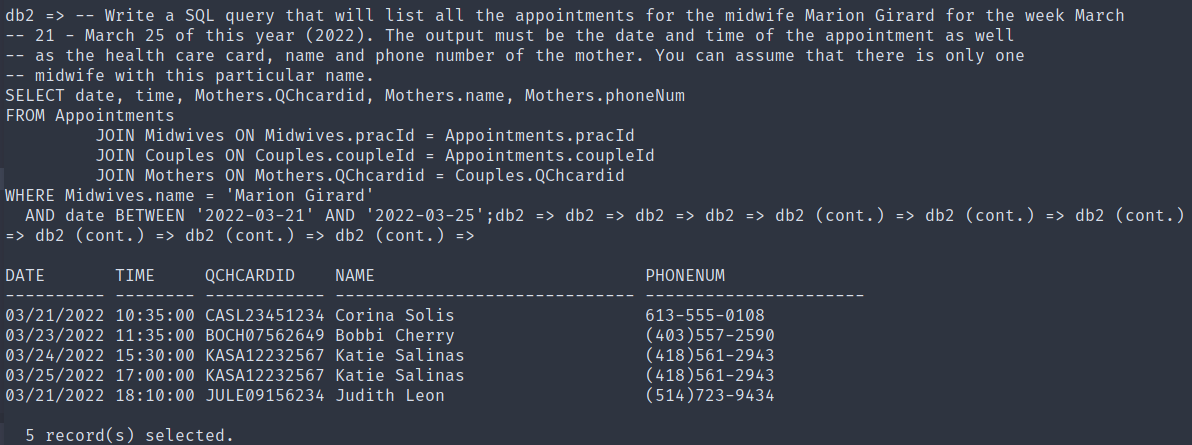
\includegraphics[scale=0.4]{5a.png}
    \caption{Q5(a)}
\end{figure}
\begin{figure}[H]
    \centering
    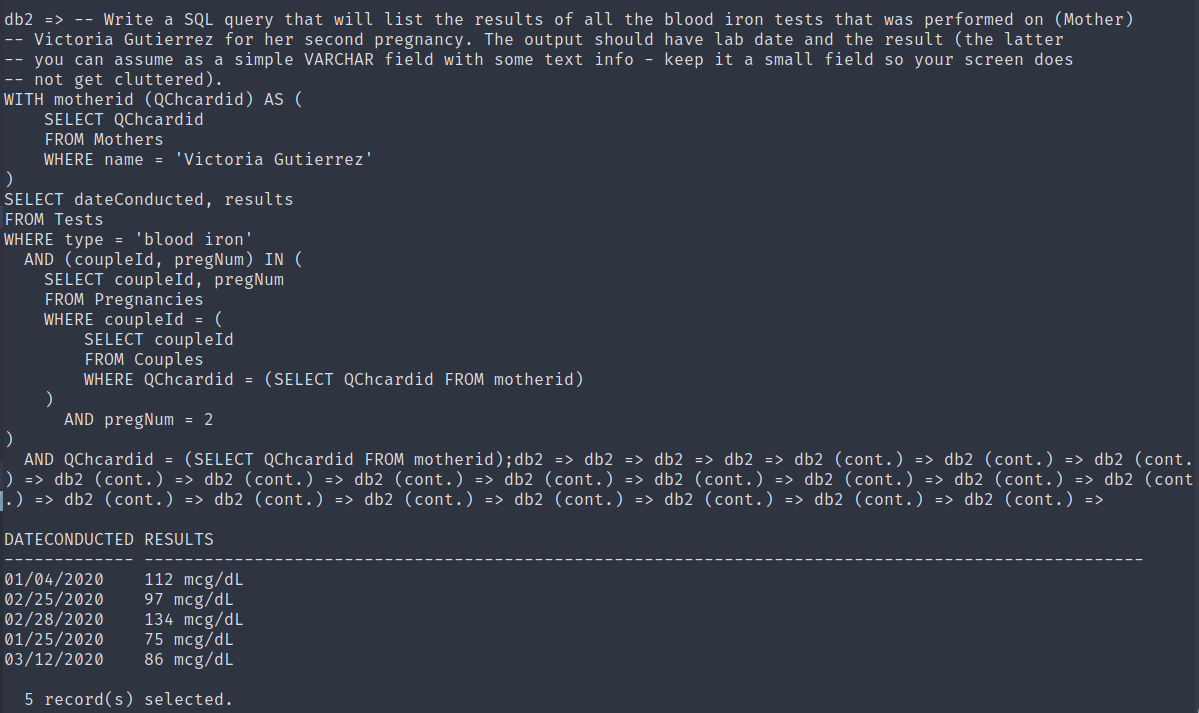
\includegraphics[scale=0.4]{5b.png}
    \caption{Q5(b)}
\end{figure}
\begin{figure}[H]
    \centering
    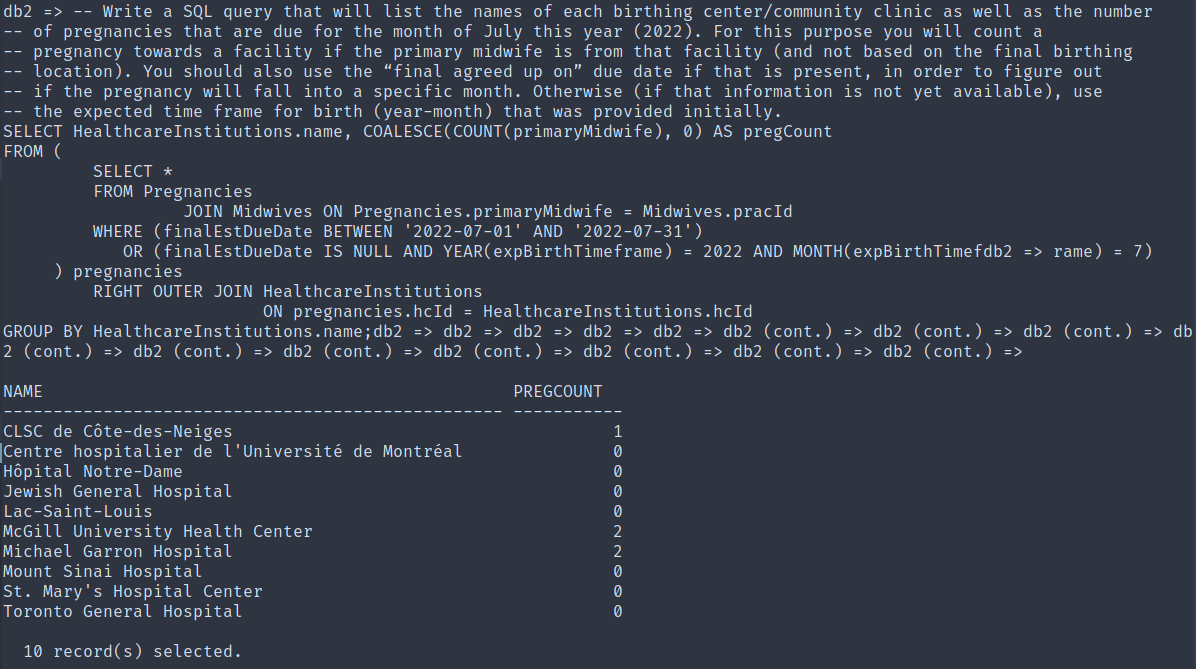
\includegraphics[scale=0.4]{5c.png}
    \caption{Q5(c)}
\end{figure}
\begin{figure}[H]
    \centering
    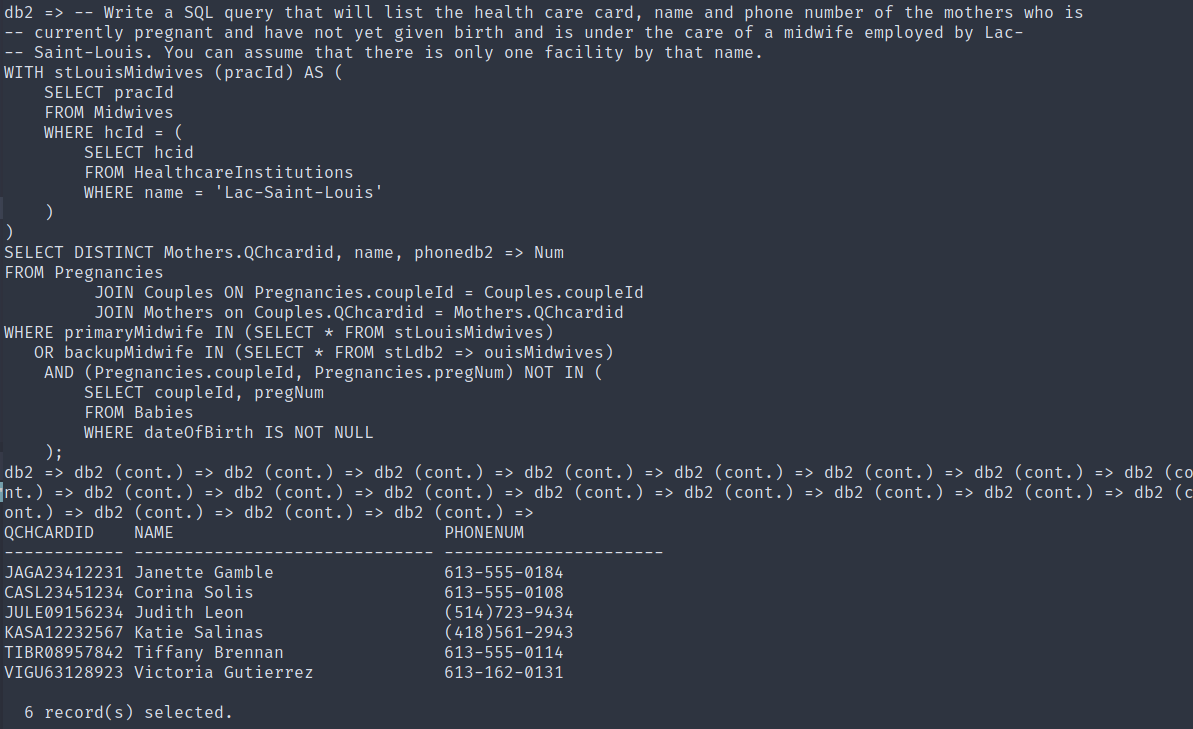
\includegraphics[scale=0.4]{5d.png}
    \caption{Q5(d)}
\end{figure}
\begin{figure}[H]
    \centering
    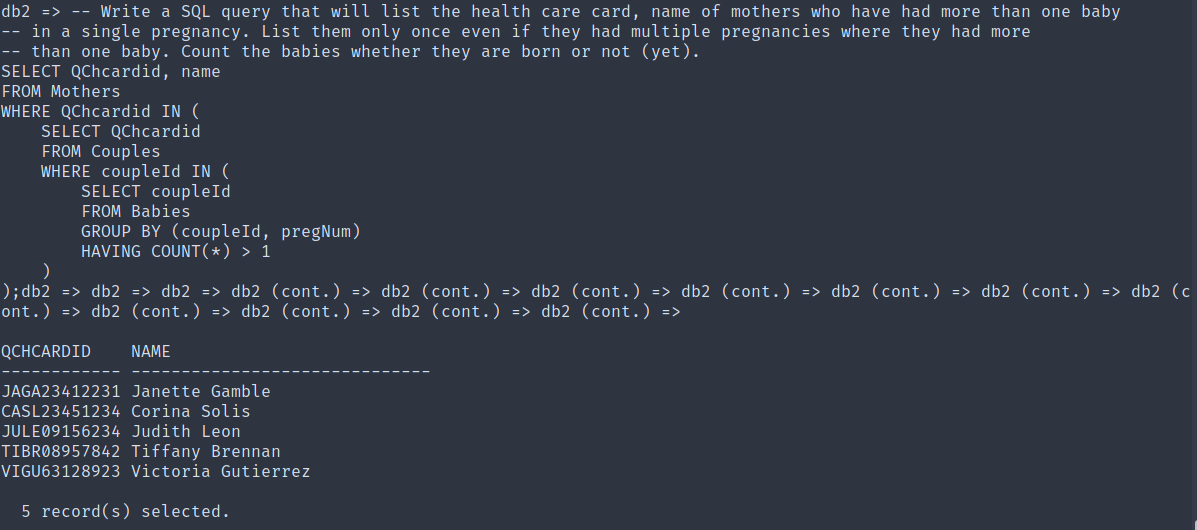
\includegraphics[scale=0.4]{5e.png}
    \caption{Q5(e)}
\end{figure}
\section*{Midwife Information}
\textbf{6 (a)}
\lstset{basicstyle=\ttfamily\normalsize,breaklines=true}
\begin{lstlisting}[language=SQL]
    CREATE VIEW midwifeinfo
    (pracId,
     name,
     phoneNum,
     email,
     InstituteName,
     InstituteAddress)
AS
SELECT pracId,
m.name,
m.phoneNum,
m.email,
hInst.name,
hInst.address
FROM Midwives m
 JOIN HealthcareInstitutions hInst on m.hcId = hInst.hcId;
\end{lstlisting}
\textbf{6 (b)}
\begin{figure}[H]
    \centering
    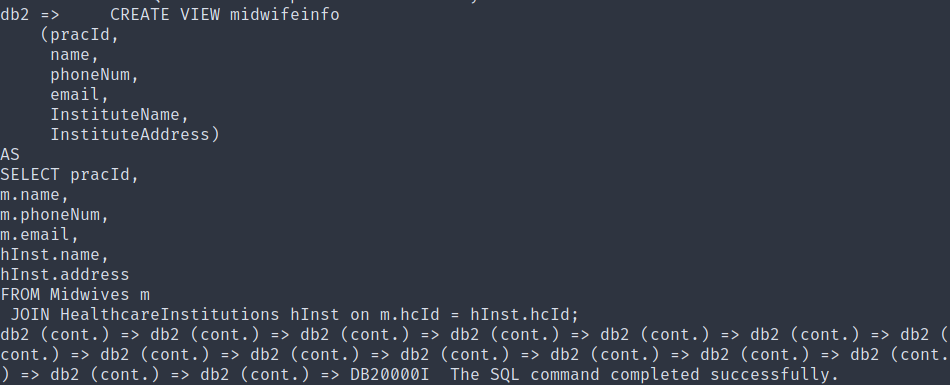
\includegraphics[scale=0.5]{view_creation.png}
    \caption{midwifeinfo view creation}
\end{figure}

\noindent\textbf{6 (c)}
\begin{figure}[H]
    \centering
    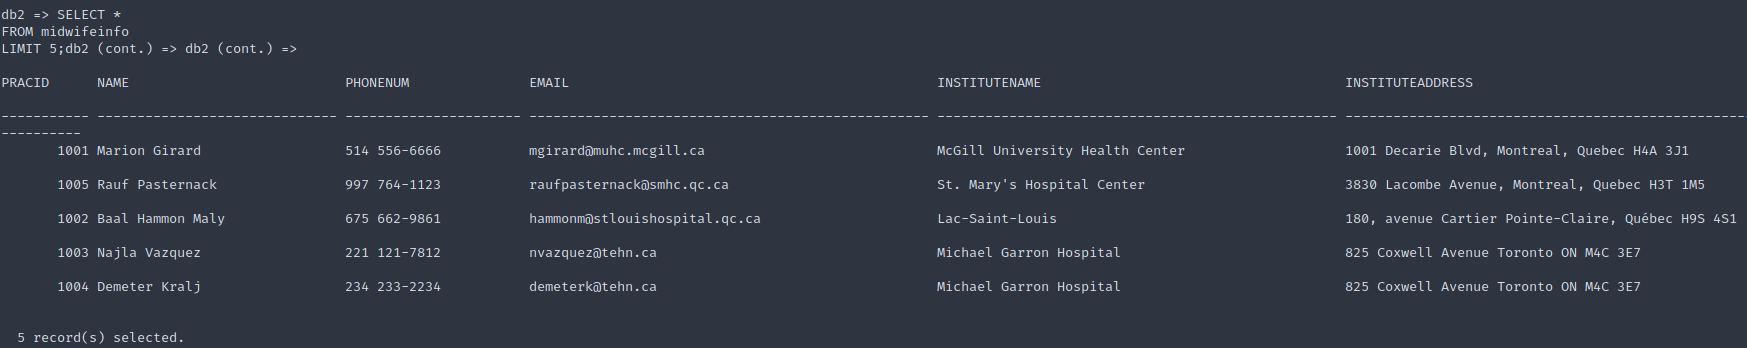
\includegraphics[scale=0.27]{viewquery.png}
    \caption{midwifeinfo view query}
\end{figure}
\noindent\textbf{6 (d)}
\begin{figure}[H]
    \centering
    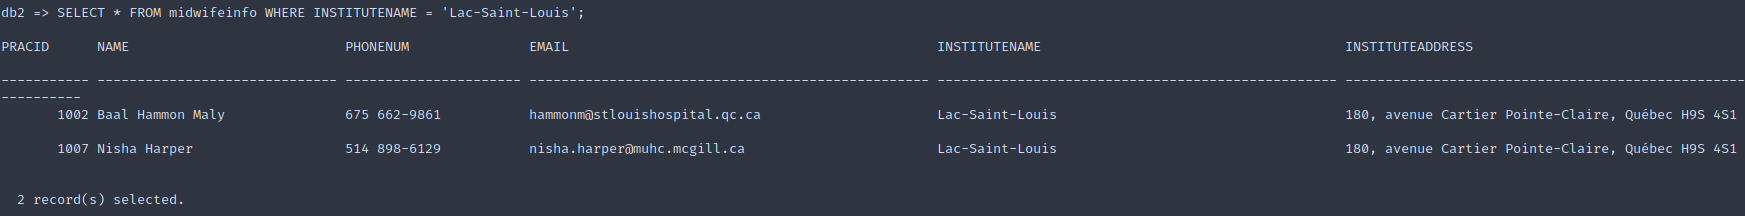
\includegraphics[scale=0.27]{viewquery2.png}
    \caption{midwifeinfo view query where on midwives employed at Lac-Saint-Louis}
\end{figure}
\noindent\textbf{6 (e)} -
Insering valid data into the view fails (as show in Figure 9).
In theory, the reason behing this is that views are unmaterialized relations, storing a query definition rather than a set of tuples and thus cannot be treated as tables and tuples cannot be inserted into them.

Insering into views is allowed in IBM DB2 (it is not only a unmaterialized relation in the DB implementation). However, the \code{midwifeinfo} view is created of two base tables \code{Midwives} and \code{HealthcareInstitutions}, that have attributes not presented in the view with \code{NOT-NULL} constraints and no default values. Therefore, inserting in the view fails. Furthermore, DB2 documentation states that \code{JOIN}s in the view definition prohibit further updates to the view, which can be yet another reason this operation fails.
\begin{figure}[H]
    \centering
    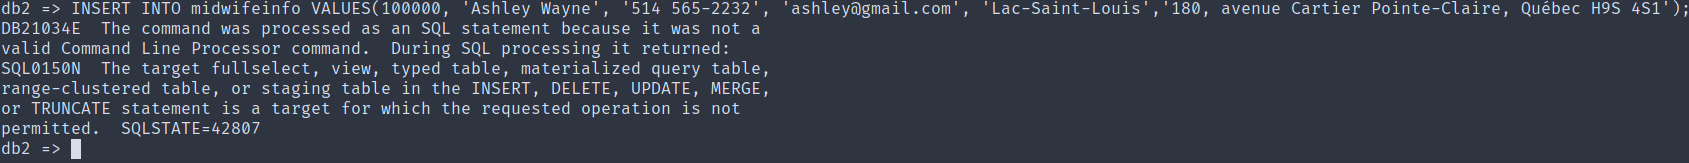
\includegraphics[scale=0.27]{viewinsertion.png}
    \caption{view insertion}
\end{figure}
\end{document}